\section{Цель работы}
Применяя разные методы, найти минимум заданного функционала.


\section{Теоретические сведения}

Функция $J(\xi)$ в точке $\xi^*$ имеет минимум, если выполняются два условия:
\begin{enumerate}
	\item Необходимое условие:
	\begin{equation}\label{need_condition}
	\cfrac{\partial{J}}{\partial{\xi}} = grad~J = 0,
	\end{equation}
	\item Достаточное условие:
	\begin{equation}\label{must_condition}
	\cfrac{\partial^2 J}{\partial{\xi^2}} > 0.
	\end{equation}
\end{enumerate}

Функция Лагранжа представляется следующим выражением:
\begin{equation}
	J_A(x,u,\lambda) = J(x,u) + \lambda \cdot c(x,u),
\end{equation}
где $J(x,u)$~-- некоторая функция, $\lambda$~-- множитель Лагранжа, $c(x, u)$~-- уравнение связи.

\section{Исходные данные}
Варианту \textnumero2 соответствует следующий набор исходных данных. 

Функционал:
\begin{equation}\label{functional}
    J(x, u) = 2 x^2 + u^2 + 2 x u + 3 x + 5 u - 10 
\end{equation}

Ограничение:
\begin{equation}\label{condition}
	c(x, u) = x - 2 u ^2
\end{equation}


\vspace{0.3cm}
\section{Поиск глобального минимума на основе необходимого и достаточного условий}
\subsection{Без ограничений}\label{global_min}
Из необходимого условия~\eqref{need_condition} экстремума функции, при $\xi = \begin{bmatrix}x & u\end{bmatrix}^T\!\!\!$:
\begin{equation}\label{grad}
		\cfrac{\partial{J}}{\partial{\xi}} = 
		\begin{bmatrix}
			4 x + 2 u + 3 \\
			2 x + 2 u + 5
		\end{bmatrix}\!\!;
\end{equation}

Составим и решим систему уравнений:
\begin{equation}
	\begin{cases}
		4 x + 2 u + 3 = 0 \\
		2 x + 2 u + 5 = 0
	\end{cases}
\end{equation}

Откуда, точка экстремума:
\begin{equation}\label{global_min_point}
	\xi^* = 
	\begin{bmatrix}
		x^*\\u^*
	\end{bmatrix}
	=
	\begin{bmatrix}
		1 \\
		-\cfrac{7}{2}~
	\end{bmatrix}
\end{equation}

Из достаточного условия~\eqref{must_condition}, запишем матрицу Гессе:
\begin{equation}\label{gesse}
	H = 
	\begin{bmatrix}
		\cfrac{\partial^2 J}{\partial x^2} & \cfrac{\partial^2 J}{\partial x \partial u} \\
		\cfrac{\partial^2 J}{\partial u \partial x} & \cfrac{\partial^2 J}{\partial u^2}
	\end{bmatrix}
	= 
	\begin{bmatrix}
		4 & 2 \\
		2 & 2
	\end{bmatrix}
\end{equation}

Так как первый и второй миноры матрицы Гессе $H$ положительны, заключаем, что точка $\xi^*	= \begin{bmatrix} 1 & -\cfrac{7}{2} \end{bmatrix}^T$~--- глобальный минимум $J(\xi)$. Поверхность заданной функции~\eqref{functional} можно увидеть на рисунке~\ref{gm}

\begin{figure}[h!]
	\centering
	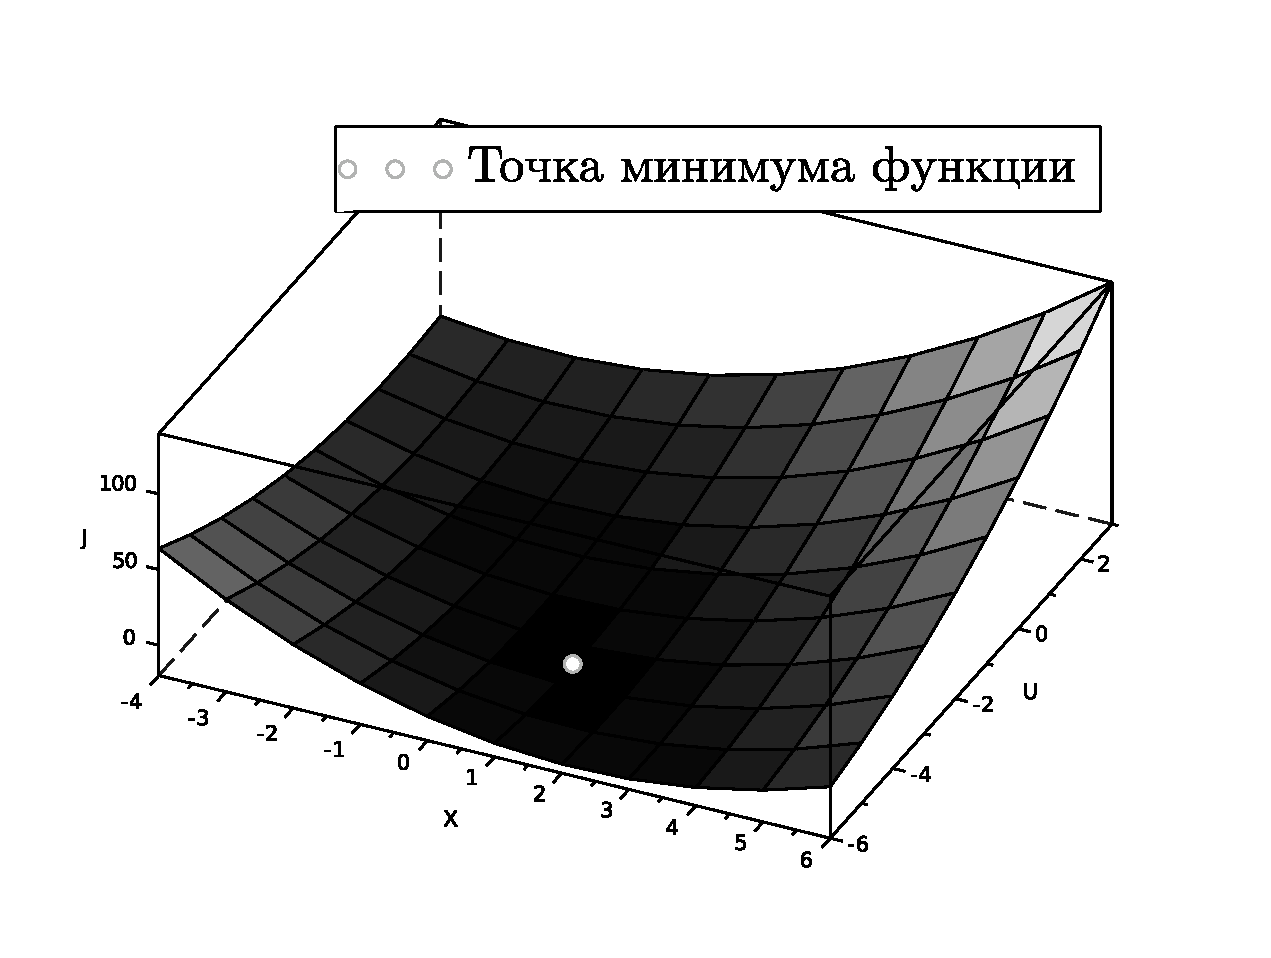
\includegraphics[width=1\textwidth]{Jux_global_minimum.pdf}
	\vspace{0cm}
	\caption{Глобальный минимум функции $J(x,u)$}}
	\label{gm}
\end{figure}

\subsection{С ограничением в виде равенства $c(x, u) = 0$}

\begin{enumerate}
	\item Первый способ решения.
	
	Выразим из ограничения~\eqref{condition} $x$:
	\begin{equation}\label{temp1}
		x = 2 u^2
	\end{equation}
	
	Подставим в~\eqref{functional}:
	\begin{equation}
		J(u) = 8 u^4 + 4 u^3 + 7 u^2 + 5 u - 10
	\end{equation}
	
	Найдем критические точки функции $J(u)$, в соответствии с необходимым	 условием~\eqref{need_condition}.
	\begin{equation}
		\cfrac{\partial J}{\partial u} = 32 u^3 + 12 u^2 + 14 u + 5 = 0
	\end{equation}

	Уравнение имеет единственный действительный корень $u = -0.3612456$, подставив который в~\eqref{temp1}, найдем $x = 0.2609967$. Таким образом, точка экстремума представляется, как:
	\begin{equation}
		\xi^* = 
		\begin{bmatrix}
			x^*\\ u^*
		\end{bmatrix}
		=
		\begin{bmatrix}
			0.2609967 \\ -0.3612456
		\end{bmatrix}
	\end{equation}
	
	Проверим достаточное условие~\eqref{must_condition} экстремума для найденной точки $\xi^*$, для это найдем частную производную второго порядка функции $J$:
	\begin{equation}
		\cfrac{\partial J}{\partial u} = 4 > 0
	\end{equation}
	
	Так как достаточное условие выполняется, заключаем, что в точке $\xi^*$ находится минимум функции $J(x, u)$.	
	
	Итак, в условиях ограничения $c(x, u) = 0$, минимум функции~\eqref{functional} равен:
	\begin{equation}
		J(x, u)_{min} = - 10.945069 
	\end{equation}

	\item Второй способ решения. Метод множителей Лагранжа.
	
	Составим расширенный критерий, записав функцию Лагранжа для заданной функции~\eqref{functional} и условия ограничения~\eqref{condition}:
	\begin{equation}\label{l_func}
		J_A(x,u,\lambda) = 2 x^2 + u^2 + 2 x u + 3 x + 5 u - 10 + \lambda (x - 2 u^2),
	\end{equation}
	
	В соответствии с необходимым условием~\eqref{condition}, найдем частные производные $J_A$:
	\begin{equation}
		\cfrac{\partial J_A}{\partial x} = 4 x + 2 u + 3 + \lambda;~\cfrac{\partial J_A}{\partial u} = 2 x + 2 u + 5 - 4 \lambda u
	\end{equation}
	
	Составим систему уравнений:
	\begin{gather}\label{nonsolving_system}
		\begin{cases}
			\cfrac{\partial J_A}{\partial x} = 0 \\
			\cfrac{\partial J_A}{\partial u} = 0 \\
			c(x, u) = 0
		\end{cases}\!\!\!;~~~
		\begin{cases}
			4 x + 2 u + 3 + \lambda = 0 \\
			2 x + 2 u + 5 - 4 \lambda u = 0 \\
			x - 2 u^2 = 0
		\end{cases}\!\!\!; \\
	\end{gather}
	
	Домножим обеи части первого уравнения на $4 u$, затем сложим первые два уравнения, а из второго выразим $x$: 
	\begin{equation}
		\begin{cases}
			16 u x + 8 u^2 + 14 u + 2 x + 5 = 0\\
			x = 2 u^2
		\end{cases}\!\!\!;
	\end{equation}	
	
	Подставляя второе в первое, в итоге получим кубическое уравнение:
	\begin{equation}
		32 u^3 + 12 u^2 + 14 u + 5 = 0,
	\end{equation}
	
	Решением которого является единственный действительный корень $u^* = -0.3612456$. Отсюда $x^* = 0.2609967$ и точка $\xi^* = \begin{bmatrix}0.2609967 \\ -0.3612456\end{bmatrix}$.
	
	Если сейчас найти $\lambda$ из первого и второго уравнений, она выйдет разной. и, если продолжить выполнять проверку подставляя полученные $u$ и $x$ в систему уравнений, то проверка не удовлетворит равенствам.
	
	Проверим полученную точку $\xi^*$ на достаточное условие. Для этого, найдем частные производные функции $J_A(x,u,\lambda)$ по $\lambda$:
	\begin{gather}
		\cfrac{\partial^2 J_A}{\partial\lambda \partial x} = 1;~~
		\cfrac{\partial^2 J_A}{\partial\lambda \partial u} = - 4 u;
	\end{gather}
	
	Также найдем частные производные второго порядка относительно аргументов $x$ и $u$:
	\begin{gather}
		\cfrac{\partial^2 J_A}{\partial x^2} = 4;~~ 0
		\cfrac{\partial^2 J_A}{\partial u^2} = 2 - 4 \lambda;~~
				\cfrac{\partial^2 J_A}{\partial x \partial u} = 2.
	\end{gather}
	
	Из полученных производных составим матрицу в виде:
	\begin{equation}
		A = 
		\begin{bmatrix}
			0 & \cfrac{\partial J_A}{\partial \lambda \partial x} & \cfrac{\partial J_A}{\partial \lambda \partial u} \\
			\cfrac{\partial J_A}{\partial \lambda \partial x} & \cfrac{\partial^2 J_A}{\partial x^2} & \cfrac{\partial^2 J_A}{\partial x \partial u}\\
			\cfrac{\partial J_A}{\partial \lambda \partial u} & \cfrac{\partial^2 J_A}{\partial u \partial x} & \cfrac{\partial^2 J_A}{ \partial u^2}
		\end{bmatrix}
		=
		\begin{bmatrix}
			0 & 1 & -4 u \\
			1 & 4 & 2 \\
			-4 u & 2 & 2 - 4 \lambda
		\end{bmatrix}
		= 
		\begin{bmatrix}
		    0 &          1 &    1.44  \\
			1 &           4 &    2 \\         
			1.44 &   2 &    15.28  
		\end{bmatrix}
	\end{equation}
	
	Найдем определитель:
	\begin{equation}
		\det{A} =  - 17.857949 < 0
	\end{equation}
	
	Следовательно, при ограничениях~\eqref{condition} функция $J_A(x,u,\lambda)$ в точке $\xi^*$ имеет минимум, равный:
	\begin{equation}
		J(x,u)_{min}=  - 10.945069 
	\end{equation}
	
	Полученная точка изображена на рисунке~\ref{gm_for_condition1}.
	
	\begin{figure}[h!]
		\centering
		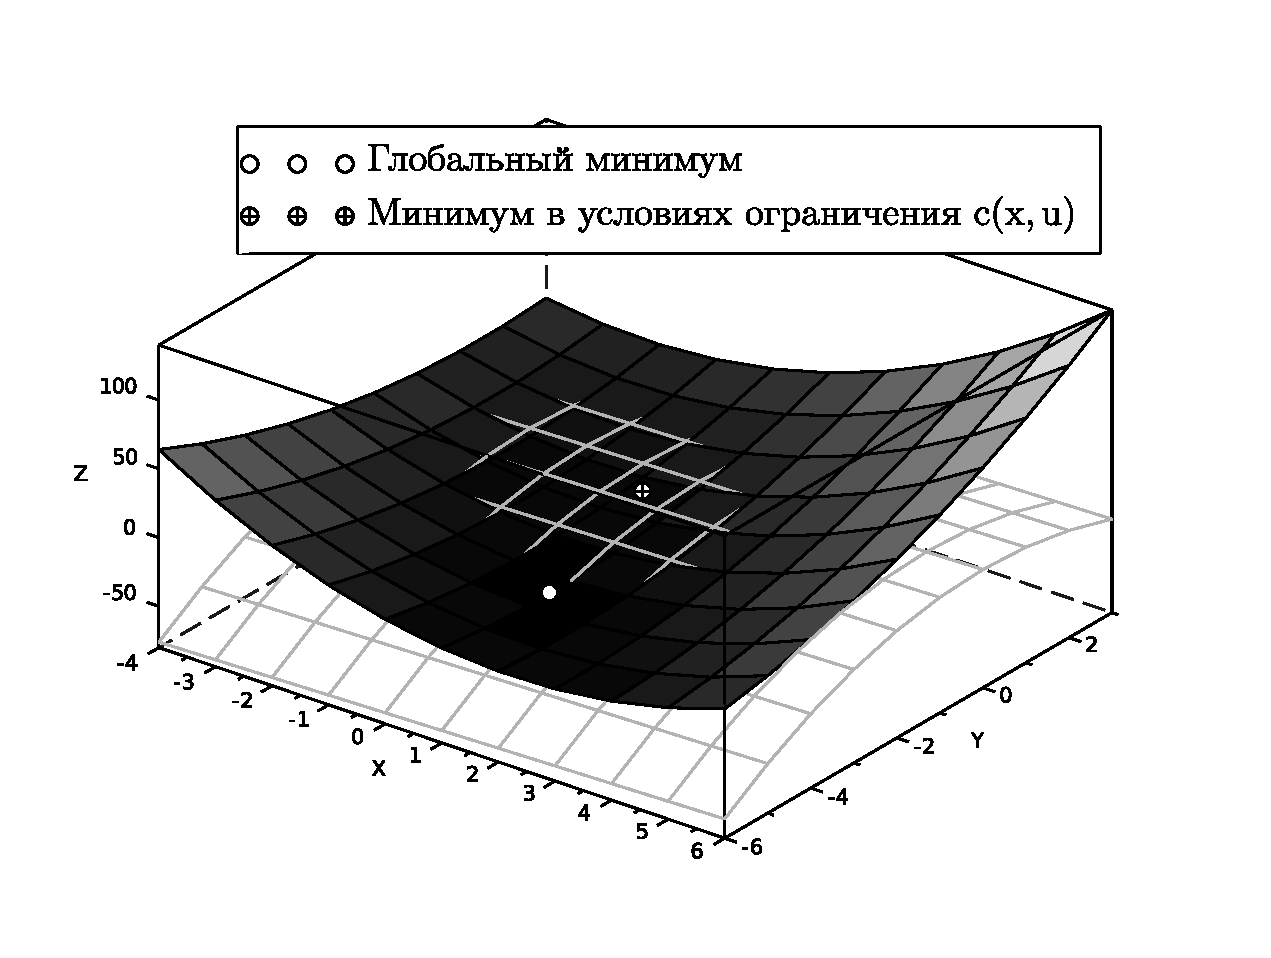
\includegraphics[width=1\textwidth]{condition_minimum.pdf}
		\vspace{0cm}
		\caption{Минимум функции $J(x,u)$ в условиях ограничения $c(x,u)$}}
		\label{gm_for_condition1}
	\end{figure}
	
\end{enumerate}


\subsection{С ограничением в виде неравенства $c(x, u) \le 0$}

Выполним проверку на ограничение в виде $c(x,u) \le 0$, для этого подставим точку глобального минимума~\eqref{global_min_point} в функцию Лагранжа~\eqref{l_func}, получим, $\lambda = 3.33$ из~\eqref{nonsolving_system}:
\begin{equation}
	J_A(x,u,\lambda) = -95.505,
\end{equation}
что не соответствует значению глобального минимума и, следовательно несправедливо для рассматриваемого ограничения.


\section{Градиентный поиск минимума критерия качества}
\subsection{Пошаговый расчет экстремума методом Ньютона-Рафсона}

Алгоритм численного поиска минимума функции~\eqref{functional} методом Ньютона-Рафсона представляется следующим выражением:
\begin{equation}\label{nr}
	\begin{bmatrix}
		x_{k+1} \\ u_{k+1}
	\end{bmatrix}
	= 
	\begin{bmatrix}
		x_k \\ u_k
	\end{bmatrix}
	-
	H^{-1} \cdot grad\,J \Big|_{x_k, u_k}
\end{equation}
где $\xi_k = \begin{bmatrix}x_k & u_k\end{bmatrix}^T\!$, $H$~--- матрица Гессе~\eqref{gesse}, $grad J$~--- градиент функции $J(x,u)$~\eqref{grad}.

Произведем инициализацию:
\begin{align*}
	\xi_0 =
	\begin{bmatrix}
		5 \\ 2
	\end{bmatrix}\!\!;~
	H^{-1} =
	\begin{bmatrix}
		\cfrac{2}{4} & -\cfrac{2}{4} \\
		-\cfrac{2}{4} & 1
	\end{bmatrix}\!\!;~
	grad\,J \Big|_{x,u}= 
	\begin{bmatrix}
	4 x + 2 u + 3 \\
	2 x + 2 u + 5
	\end{bmatrix}\!\!.
\end{align*}

Будем применять выражение~\eqref{nr} для $k \ge 0$, пока $grad\,J \ne 0$. 

Для \fbox{$k = 0$}\,:
\begin{equation}
	grad\,J \Big|_{10, 10}	
	= 
	\begin{bmatrix}
		27 \\ 19
	\end{bmatrix}
\end{equation}

\begin{align*}
	\begin{bmatrix}
		x_{1} \\ u_{1}
	\end{bmatrix}
	=
	\begin{bmatrix}
		5 \\ 2
	\end{bmatrix}
	-
	\textstyle
	\begin{bmatrix}
		\frac{2}{4} & -\frac{2}{4} \\
		-\frac{2}{4} & 1
	\end{bmatrix}
	\cdot
	\begin{bmatrix}
		27 \\ 19
	\end{bmatrix}
	=
	\begin{bmatrix}
		5 \\ 2
	\end{bmatrix}
	-
	\begin{bmatrix}
		13.5-9.5 \\ -13.5 + 19
	\end{bmatrix}
	= 
	\begin{bmatrix}
		5 - 4 \\ 2 - 5.5
	\end{bmatrix}
	= 
	\begin{bmatrix}
		1 \\ -3.5
	\end{bmatrix}	
\end{align*}

Для \fbox{$k = 1$}\,, получаем:
\begin{equation}
	grad\,J \Big|_{-15, 14}	
	= 
	\begin{bmatrix}
		0 \\ 0
	\end{bmatrix}
\end{equation}

Итак, так как градиент в найденной точке равен нулю, заключаем, что нашли точку экстремума $\xi^*(1, -3.5)$ функции~\eqref{functional}, что полностью совпадает с решением из пункта~\ref{global_min}. Графическую интерпретацию поиска этой точки можно увидеть на рисунке~\ref{NR}

\begin{figure}[h!]
	\begin{minipage}[h]{0.5\linewidth}
		\center{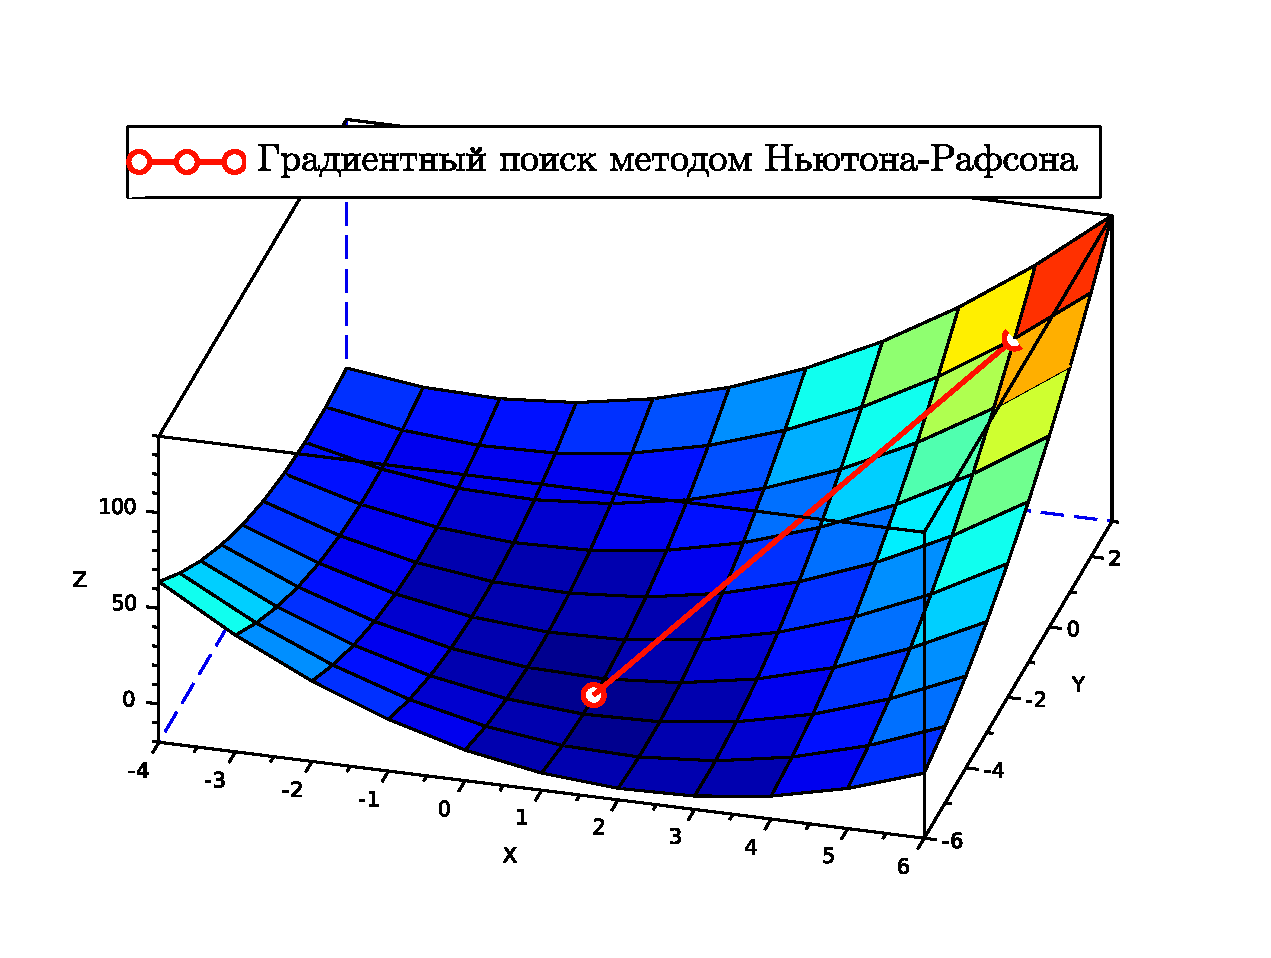
\includegraphics[width=1\linewidth]{NR3d.pdf}}
	\end{minipage}
	\hfill
	\begin{minipage}[h]{0.5\linewidth}
		\center{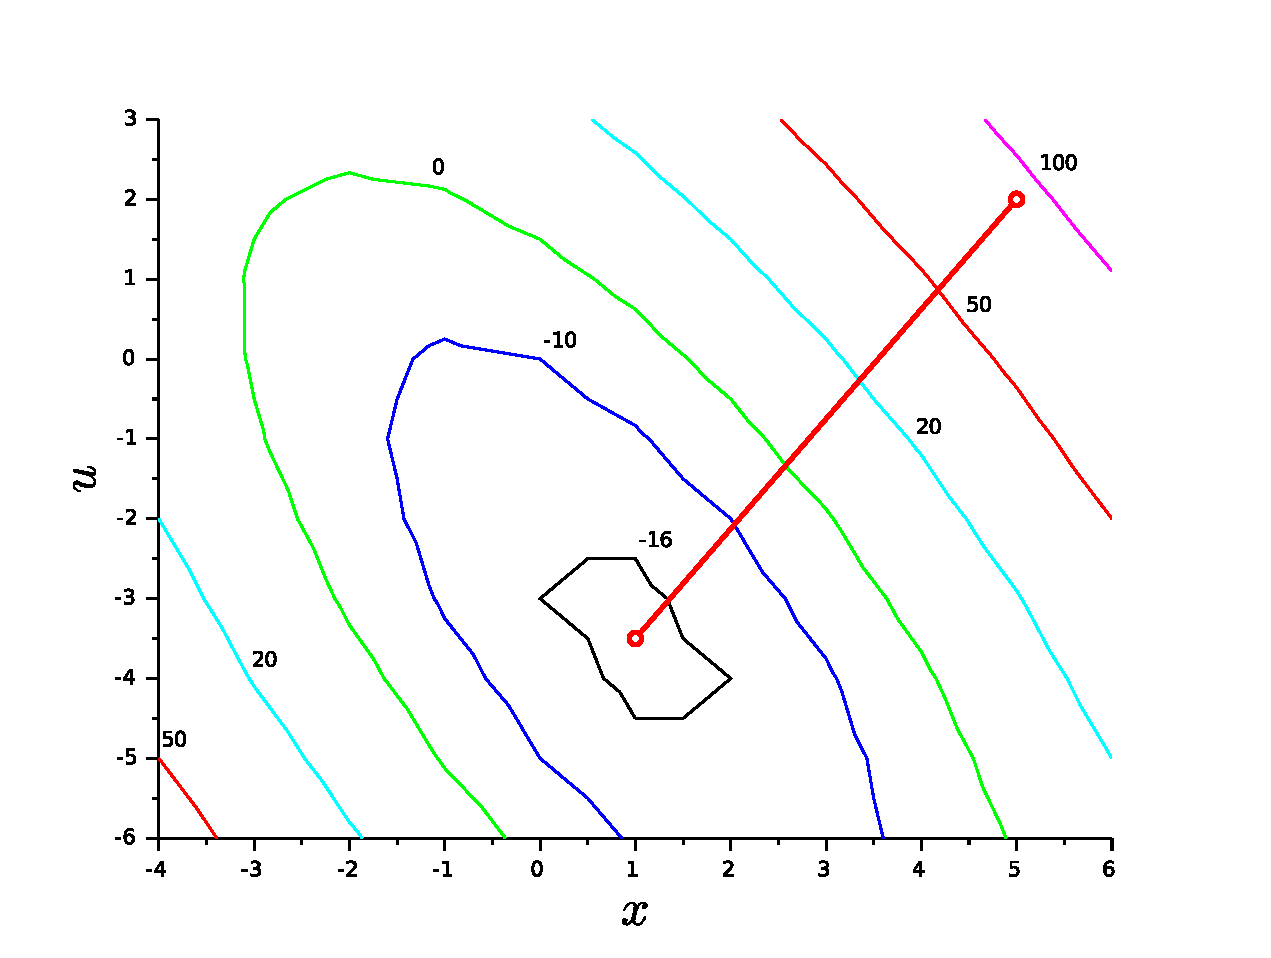
\includegraphics[width=1\linewidth]{NR2d.pdf}}
	\end{minipage}
	\caption{Графическая интерпретация метода Ньютона"---~Рафсона}
	\label{NR}
\end{figure}


\subsection{Пошаговый расчет экстремума методом наискорейшего спуска}
Алгоритм численного поиска минимума функции~\eqref{functional} методом наискорейшего спуска представляется следующим выражением:
\begin{equation}\label{fd}
	\begin{bmatrix}
	x_{k+1} \\ u_{k+1}
	\end{bmatrix}
	= 
	\begin{bmatrix}
	x_k \\ u_k
	\end{bmatrix}
	-
	\gamma \cdot grad\,J \Big|_{x_k, u_k}
\end{equation}
где $\xi_k = \begin{bmatrix}x_k & u_k\end{bmatrix}^T\!$, $\gamma$~--- коэффициент скорости поиска, $grad J$~--- градиент функции $J(x,u)$~\eqref{grad}.

Произведем инициализацию:
\begin{align*}
	\xi_0 =
	\begin{bmatrix}
	5 \\ 2
	\end{bmatrix}\!\!;~
	grad\,J \Big|_{x,u}= 
	\begin{bmatrix}
	4 x + 2 u + 3 \\
	2 x + 2 u + 5
	\end{bmatrix}\!\!.
\end{align*}

Будем применять выражение~\eqref{fd} для $k \ge 0$, пока $grad\,J \ne 0$. 

\begin{enumerate}
	\item \fcolorbox{green}{lgreen}{$\gamma = 0.3$ -- колебательная сходимость.}
	
	Для \fbox{$k = 0$}\,:
	\begin{align*}
		\begin{bmatrix}
			x_{1} \\ u_{1}
		\end{bmatrix}
		=
		\begin{bmatrix}
			5 \\ 2
		\end{bmatrix}
		-
		0.3
		\begin{bmatrix}
		27 \\ 19
		\end{bmatrix}
		=
		\begin{bmatrix}
		5 - 8.1 \\ 2 - 5.7
		\end{bmatrix}
		= 
		\begin{bmatrix}
		-3.1 \\ -3.7
		\end{bmatrix}	
	\end{align*}
	
	Для \fbox{$k = 1$}\,:
	\begin{align*}
		\begin{bmatrix}
			x_{2} \\ u_{2}
		\end{bmatrix}
		=
		\begin{bmatrix}
			-3.1 \\ -3.7
		\end{bmatrix}
		-
		0.3
		\begin{bmatrix}
			-16.8 \\ -8.6
		\end{bmatrix}
		=
		\begin{bmatrix}
			-3.1 + 16.8 \\ -3.7 + 2.58
		\end{bmatrix}
		= 
		\begin{bmatrix}
			1.94 \\ -1.12
		\end{bmatrix}	
	\end{align*}

	Для \fbox{$k = 2$}\,:
	\begin{align*}
		\begin{bmatrix}
			x_{3} \\ u_{3}
		\end{bmatrix}
		=
		\begin{bmatrix}
			1.94\\
			-1.12
		\end{bmatrix}
		-
		0.3
		\begin{bmatrix}
		   8.52 \\
		   6.64
		\end{bmatrix}
		=
		\begin{bmatrix}
			-1.94 + 0.616 \\ -1.12 + 3.112
		\end{bmatrix}
		= 
		\begin{bmatrix}
			-0.616 \\ -3.112
		\end{bmatrix}	
	\end{align*}
	
	Для \fbox{$k = 3$}\,:
	\begin{align*}
		\begin{bmatrix}
		x_{4} \\ u_{4}
		\end{bmatrix}
		=
		\begin{bmatrix}
  			-0.616\\
			-3.112
		\end{bmatrix}
		-
		0.3
		\begin{bmatrix}
		  -5.688 \\
		  -2.456
		\end{bmatrix}
		=
		\begin{bmatrix}
			-0.616 - 1.0904 \\ -3.112 +2.3752
		\end{bmatrix}
		= 
		\begin{bmatrix}
			-1.0904 \\ -2.3752
		\end{bmatrix}	
	\end{align*}
	
	Для \fbox{$k = 4$}\,:
	\begin{align*}
		\begin{bmatrix}
		x_{5} \\ u_{5}
		\end{bmatrix}
		=
		\begin{bmatrix}
			1.0904 \\
			-2.3752
		\end{bmatrix}
		-
		0.3
		\begin{bmatrix}
			2.6112 \\
			2.4304
		\end{bmatrix}
		=
		\begin{bmatrix}
			1.0904 - 0.7833 \\ -2.3752 - 0.72912 
		\end{bmatrix}
		= 
		\begin{bmatrix}
			0.30704 \\ -3.10432
		\end{bmatrix}	
	\end{align*}
	
	Для \fbox{$k = 5$}\,:
	\begin{align*}
		\begin{bmatrix}
			x_{6} \\ u_{6}
		\end{bmatrix}
		=
		\begin{bmatrix}
		   0.30704 \\
		  -3.10432
		\end{bmatrix}
		-
		0.3
		\begin{bmatrix}
			-1.98048 \\
			-0.59456
		\end{bmatrix}
		=
		\begin{bmatrix}
			0.30704 + 0.5941 \\ -3.10432 + 0.1783
		\end{bmatrix}
		= 
		\begin{bmatrix}
			0.9011 \\ -2.9259
		\end{bmatrix}	
	\end{align*}

	Для \fbox{$k = 6$}\,:
	\begin{align*}
		\begin{bmatrix}
		x_{7} \\ u_{7}
		\end{bmatrix}
		=
		\begin{bmatrix}
		   0.901184 \\
		  -2.925952
		\end{bmatrix}
		-
		0.3
		\begin{bmatrix}
			   0.752832 \\
			0.950464
		\end{bmatrix}
		=
		\begin{bmatrix}
			0.901184 - 0.2258 \\ -2.9259 - 0.2851
		\end{bmatrix}
		= 
		\begin{bmatrix}
			0.6753 \\ -3.21109
		\end{bmatrix}	
	\end{align*}

	Для \fbox{$k = 7$}\,:
	\begin{align*}
		\begin{bmatrix}
			x_{8} \\ u_{8}
		\end{bmatrix}
		=
		\begin{bmatrix}
			0.6753344\\
			-3.2110912
		\end{bmatrix}
		-
		0.3
		\begin{bmatrix}
			-0.7208448 \\
			-0.0715136
		\end{bmatrix}
		=
		\begin{bmatrix}
			0.6753 + 0.2162 \\ -3.21109 + 0.0214
		\end{bmatrix}
		= 
		\begin{bmatrix}
			0.8915878\\
			-3.1896371
		\end{bmatrix}	
	\end{align*}

	Подобные шаги повторяются для $k = \overline{8,135}$, где при \fbox{$k = 135$}\,:
	\begin{align*}
		\begin{bmatrix}
			x_{136} \\ u_{136}
		\end{bmatrix}
		=
		\begin{bmatrix}
			   1\\
			-3.5
		\end{bmatrix}
		-
		0.3
		\begin{bmatrix}
			0 \\ 0
		\end{bmatrix}
		=
		\begin{bmatrix}
			1\\
			-3.5
		\end{bmatrix}
	\end{align*}

	Градиент принимает значение равное нулю, следовательно точка $\xi^*(x_{136}, u_{136})$~--- точка минимума функции $J(x,u)$. На рисунке~\ref{FD_3} изображены шаги поиска минимума с колебательной сходимостью.

	\begin{figure}[h!]
		\begin{minipage}[h]{0.5\linewidth}
			\center{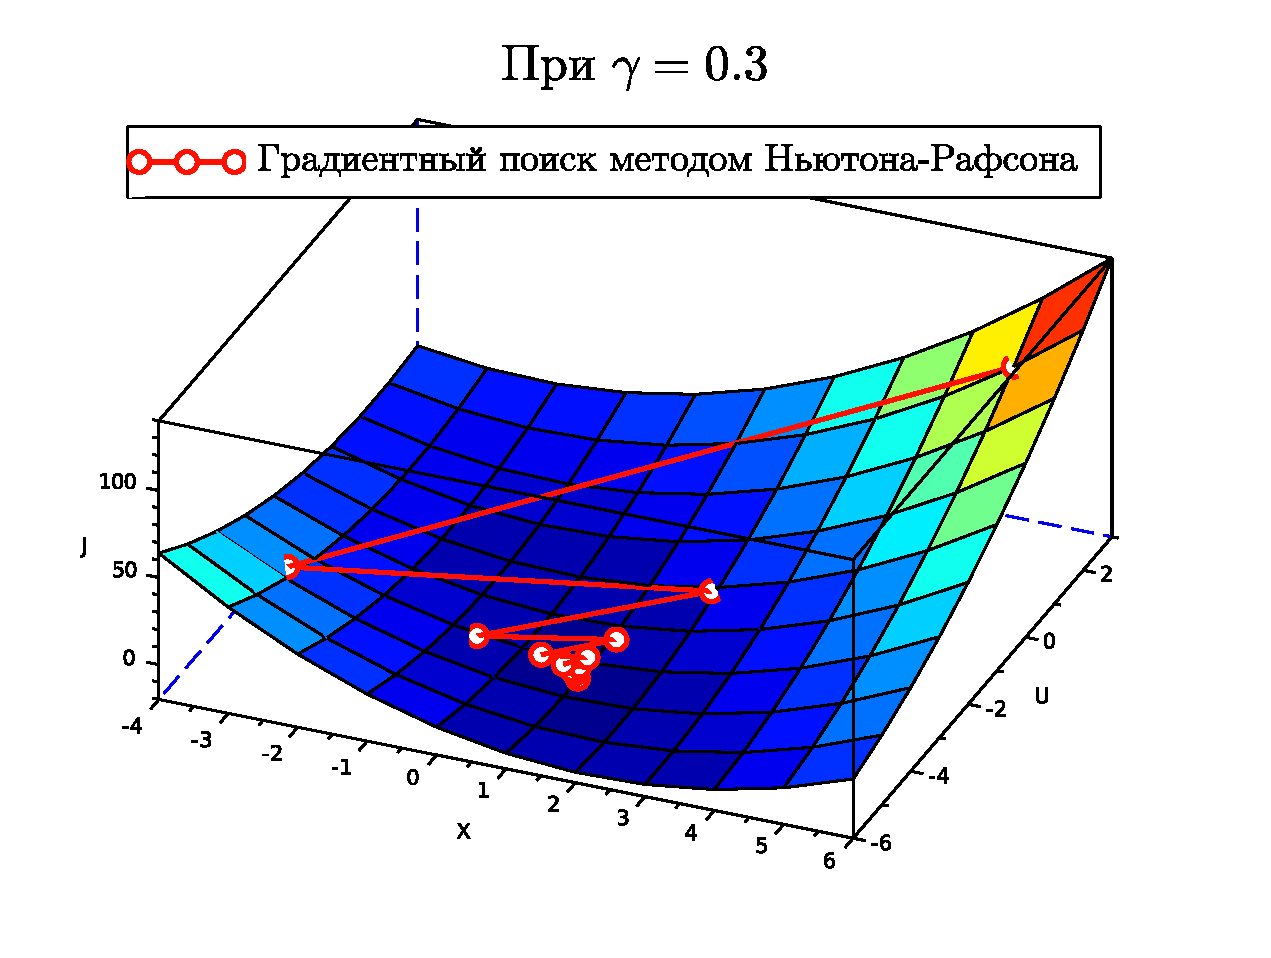
\includegraphics[width=1\linewidth]{FD3d_3.pdf}}
		\end{minipage}
		\hfill
		\begin{minipage}[h]{0.5\linewidth}
			\center{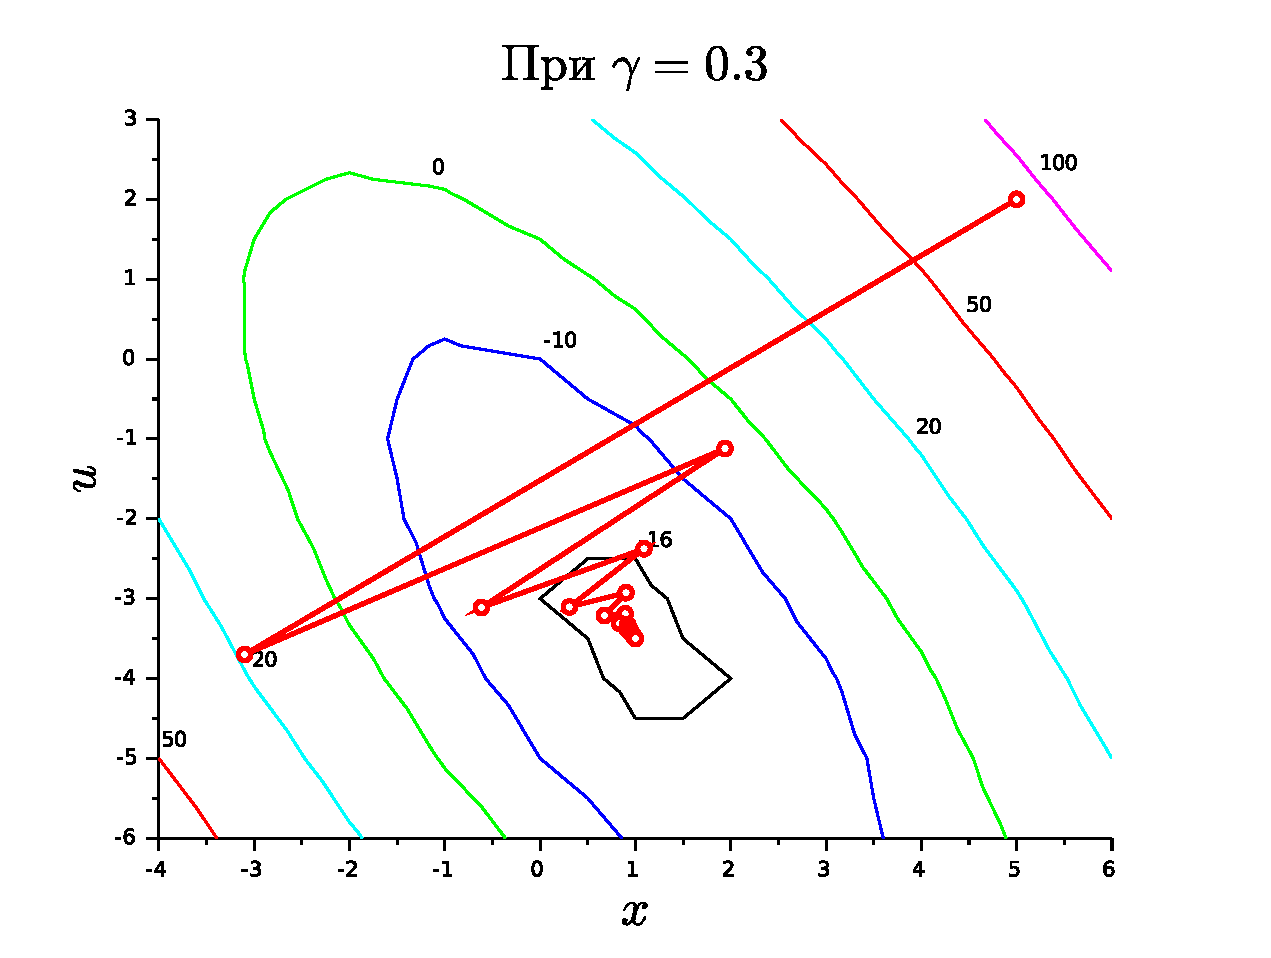
\includegraphics[width=1\linewidth]{FD2d_3.pdf}}
		\end{minipage}
		\caption{Графическая интерпретация метода Ньютона-Рафсона}
		\label{FD_3}
	\end{figure}

	\item \fcolorbox{green}{lgreen}{$\gamma = 0.01$ -- апериодическая сходимость.}
	
	Для \fbox{$k = 0$}\,:
	\begin{align*}
		\begin{bmatrix}
			x_{1} \\ u_{1}
		\end{bmatrix}
		=
		\begin{bmatrix}
			5 \\ 2
		\end{bmatrix}
		-
		0.3
		\begin{bmatrix}
			27 \\ 19
		\end{bmatrix}
		=
		\begin{bmatrix}
			5 - 0.27 \\ 2 - 19
		\end{bmatrix}
		= 
		\begin{bmatrix}
			4.73 \\
			1.81
		\end{bmatrix}	
	\end{align*}
	
	Для \fbox{$k = 1$}\,:
	\begin{align*}
		\begin{bmatrix}
			x_{2} \\ u_{2}
		\end{bmatrix}
		=
		\begin{bmatrix}
			4.73 \\
			1.81
		\end{bmatrix}
		-
		0.3
		\begin{bmatrix}
			25.54 \\
			18.08
		\end{bmatrix}
		=
		\begin{bmatrix}
			4.73 - 0.255\\
			1.81 - 18.08
		\end{bmatrix}
		= 
		\begin{bmatrix}
			4.474 \\
			1.629
		\end{bmatrix}	
	\end{align*}
	
	Для \fbox{$k = 2$}\,:
	\begin{align*}
		\begin{bmatrix}
		x_{3} \\ u_{3}
		\end{bmatrix}
		=
		\begin{bmatrix}
			4.474 \\
			1.629
		\end{bmatrix}
		-
		0.3
		\begin{bmatrix}
			24.156 \\
			17.207
		\end{bmatrix}
		=
		\begin{bmatrix}
			4.474 - 0.241\\
			1.629 - 0.172
		\end{bmatrix}
		= 
		\begin{bmatrix}
			4.233 \\
			1.457
		\end{bmatrix}	
	\end{align*}
	
	Для \fbox{$k = 3$}\,:
	\begin{align*}
		\begin{bmatrix}
			x_{4} \\ u_{4}
		\end{bmatrix}
		=
		\begin{bmatrix}
			4.233 \\
			1.457
		\end{bmatrix}
		-
		0.3
		\begin{bmatrix}
			22.846 \\
			16.38
		\end{bmatrix}
		=
		\begin{bmatrix}
			4.233 - 0.228 \\
			1.457 - 0.163
		\end{bmatrix}
		= 
		\begin{bmatrix}
			4.004 \\
			1.293
		\end{bmatrix}	
	\end{align*}
	
	Для \fbox{$k = 4$}\,:
	\begin{align*}
		\begin{bmatrix}
			x_{5} \\ u_{5}
		\end{bmatrix}
		=
		\begin{bmatrix}
			4.004 \\
			1.293
		\end{bmatrix}
		-
		0.3
		\begin{bmatrix}
			21.604 \\
			15.595
		\end{bmatrix}
		=
		\begin{bmatrix}
			4.004 - 0.216 \\
			1.293 - 0.155
		\end{bmatrix}
		= 
		\begin{bmatrix}
			3.788 \\
			1.137
		\end{bmatrix}	
	\end{align*}
	
	И так $4131$ раз, где при \fbox{$k = 4130$}\,:
	\begin{align*}
		\begin{bmatrix}
			x_{4131} \\ u_{4131}
		\end{bmatrix}
		=
		\begin{bmatrix}
			   1 \\
			-3.5
		\end{bmatrix}
		-
		0.3
		\begin{bmatrix}
			0 \\ 0
		\end{bmatrix}
		=
		\begin{bmatrix}
			1 \\ -3.5
		\end{bmatrix}	
	\end{align*}

	Градиент принимает значение равное нулю, следовательно точка $\xi^*(x_{4131}, u_{4131})$~--- точка минимума функции $J(x,u)$. На рисунке~\ref{FD_01} изображены шаги поиска минимума с апериодической сходимостью.
	
	\begin{figure}[h!]
	\begin{minipage}[h]{0.5\linewidth}
		\center{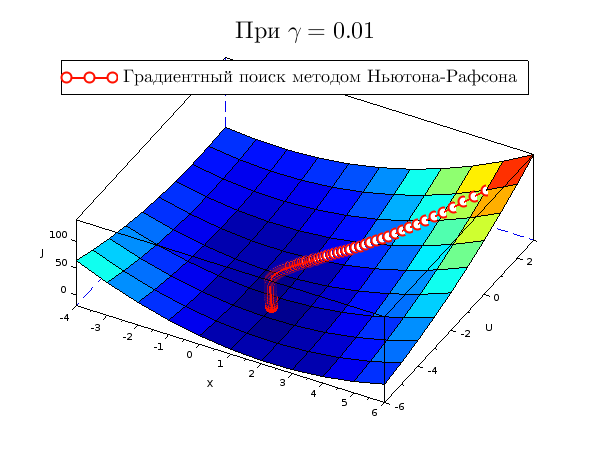
\includegraphics[width=1\linewidth]{FD3d_01.png}}
	\end{minipage}
	\hfill
	\begin{minipage}[h]{0.5\linewidth}
		\center{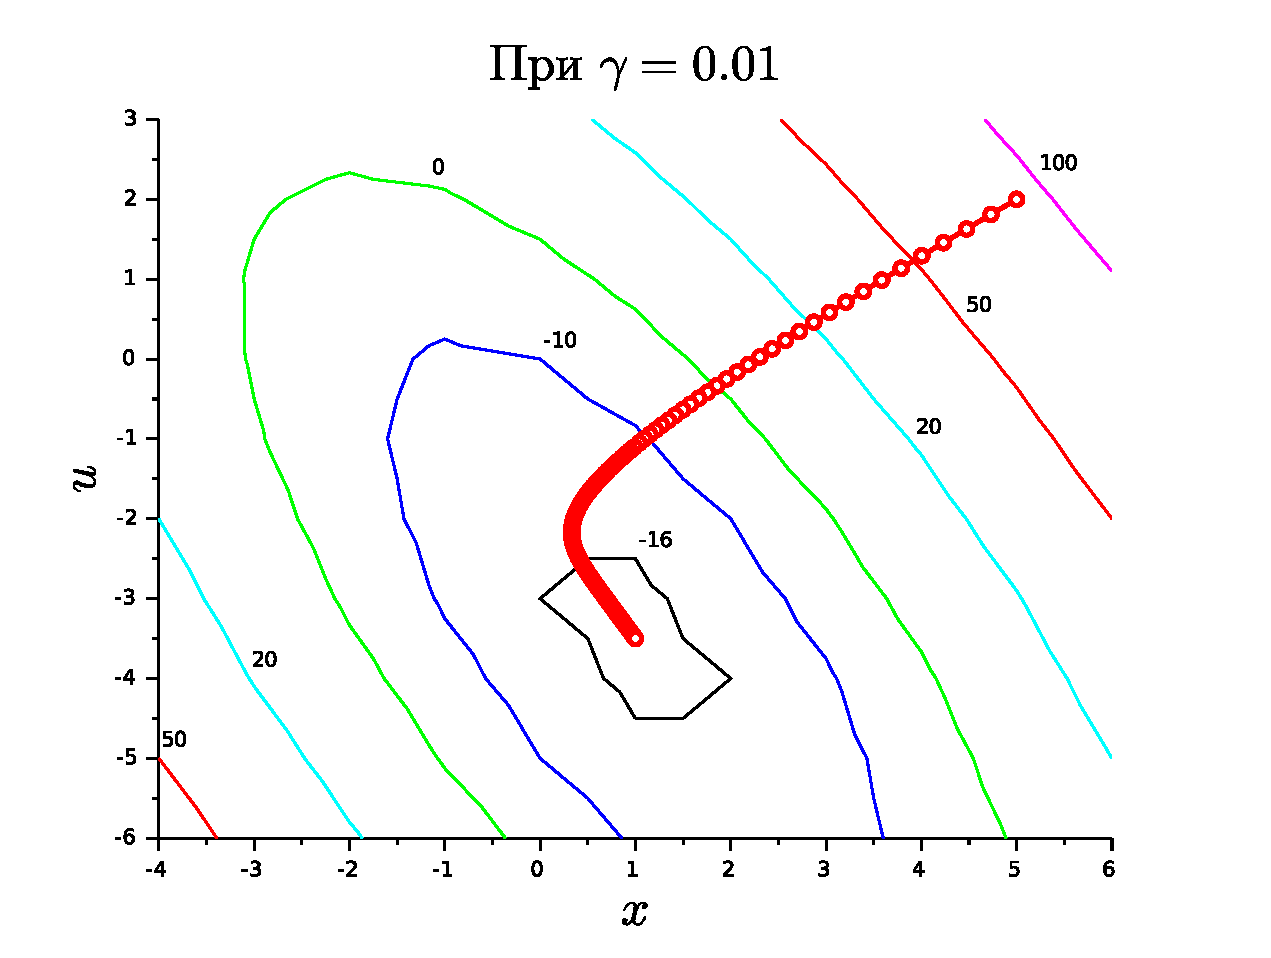
\includegraphics[width=1\linewidth]{FD2d_01.pdf}}
	\end{minipage}
	\caption{Графическая интерпретация метода наискорейшего спуска}
	\label{FD_01}
	\end{figure}		
\end{enumerate}


\newpage


\section{Выводы по работе}
В~результате проделанной работы были:
\begin{enumerate}
	\item найдены минимумы критерия качества заданной функции~\eqref{functional} как безусловные, так и в условиях заданного ограничения~\eqref{condition}. Построены соответствующие поверхности, на которых отмечены соответствующие точки разыскиваемых экстремумов, рисунки~\ref{gm}"--~4.2.
	\item пошагово выполнены два метода градиентного поиска минимума: метод Ньэтона"--~Рафсона и метод наискорейшего спуска. Выполнены необходимые для максимальной наглядности построения, рисунки~\ref{NR}"--~\ref{FD_01}.
\end{enumerate}